\documentclass{ximera}

 

\usepackage{epsfig}

\graphicspath{
  {./}
  {figures/}
}

\usepackage{morewrites}
\makeatletter
\newcommand\subfile[1]{%
\renewcommand{\input}[1]{}%
\begingroup\skip@preamble\otherinput{#1}\endgroup\par\vspace{\topsep}
\let\input\otherinput}
\makeatother

\newcommand{\includeexercises}{\directlua{dofile("/home/jim/linearAlgebra/laode/exercises.lua")}}

%\newcounter{ccounter}
%\setcounter{ccounter}{1}
%\newcommand{\Chapter}[1]{\setcounter{chapter}{\arabic{ccounter}}\chapter{#1}\addtocounter{ccounter}{1}}

%\newcommand{\section}[1]{\section{#1}\setcounter{thm}{0}\setcounter{equation}{0}}

%\renewcommand{\theequation}{\arabic{chapter}.\arabic{section}.\arabic{equation}}
%\renewcommand{\thefigure}{\arabic{chapter}.\arabic{figure}}
%\renewcommand{\thetable}{\arabic{chapter}.\arabic{table}}

%\newcommand{\Sec}[2]{\section{#1}\markright{\arabic{ccounter}.\arabic{section}.#2}\setcounter{equation}{0}\setcounter{thm}{0}\setcounter{figure}{0}}

\newcommand{\Sec}[2]{\section{#1}}

\setcounter{secnumdepth}{2}
%\setcounter{secnumdepth}{1} 

%\newcounter{THM}
%\renewcommand{\theTHM}{\arabic{chapter}.\arabic{section}}

\newcommand{\trademark}{{R\!\!\!\!\!\bigcirc}}
%\newtheorem{exercise}{}

\newcommand{\dfield}{{\sf dfield9}}
\newcommand{\pplane}{{\sf pplane9}}

\newcommand{\EXER}{\section*{Exercises}}%\vspace*{0.2in}\hrule\small\setcounter{exercise}{0}}
\newcommand{\CEXER}{}%\vspace{0.08in}\begin{center}Computer Exercises\end{center}}
\newcommand{\TEXER}{} %\vspace{0.08in}\begin{center}Hand Exercises\end{center}}
\newcommand{\AEXER}{} %\vspace{0.08in}\begin{center}Hand Exercises\end{center}}

% BADBAD: \newcommand{\Bbb}{\bf}

\newcommand{\R}{\mbox{$\Bbb{R}$}}
\newcommand{\C}{\mbox{$\Bbb{C}$}}
\newcommand{\Z}{\mbox{$\Bbb{Z}$}}
\newcommand{\N}{\mbox{$\Bbb{N}$}}
\newcommand{\D}{\mbox{{\bf D}}}
\usepackage{amssymb}
%\newcommand{\qed}{\hfill\mbox{\raggedright$\square$} \vspace{1ex}}
%\newcommand{\proof}{\noindent {\bf Proof:} \hspace{0.1in}}

\newcommand{\setmin}{\;\mbox{--}\;}
\newcommand{\Matlab}{{M\small{AT\-LAB}} }
\newcommand{\Matlabp}{{M\small{AT\-LAB}}}
\newcommand{\computer}{\Matlab Instructions}
\newcommand{\half}{\mbox{$\frac{1}{2}$}}
\newcommand{\compose}{\raisebox{.15ex}{\mbox{{\scriptsize$\circ$}}}}
\newcommand{\AND}{\quad\mbox{and}\quad}
\newcommand{\vect}[2]{\left(\begin{array}{c} #1_1 \\ \vdots \\
 #1_{#2}\end{array}\right)}
\newcommand{\mattwo}[4]{\left(\begin{array}{rr} #1 & #2\\ #3
&#4\end{array}\right)}
\newcommand{\mattwoc}[4]{\left(\begin{array}{cc} #1 & #2\\ #3
&#4\end{array}\right)}
\newcommand{\vectwo}[2]{\left(\begin{array}{r} #1 \\ #2\end{array}\right)}
\newcommand{\vectwoc}[2]{\left(\begin{array}{c} #1 \\ #2\end{array}\right)}

\newcommand{\ignore}[1]{}


\newcommand{\inv}{^{-1}}
\newcommand{\CC}{{\cal C}}
\newcommand{\CCone}{\CC^1}
\newcommand{\Span}{{\rm span}}
\newcommand{\rank}{{\rm rank}}
\newcommand{\trace}{{\rm tr}}
\newcommand{\RE}{{\rm Re}}
\newcommand{\IM}{{\rm Im}}
\newcommand{\nulls}{{\rm null\;space}}

\newcommand{\dps}{\displaystyle}
\newcommand{\arraystart}{\renewcommand{\arraystretch}{1.8}}
\newcommand{\arrayfinish}{\renewcommand{\arraystretch}{1.2}}
\newcommand{\Start}[1]{\vspace{0.08in}\noindent {\bf Section~\ref{#1}}}
\newcommand{\exer}[1]{\noindent {\bf \ref{#1}}}
\newcommand{\ans}{}
\newcommand{\matthree}[9]{\left(\begin{array}{rrr} #1 & #2 & #3 \\ #4 & #5 & #6
\\ #7 & #8 & #9\end{array}\right)}
\newcommand{\cvectwo}[2]{\left(\begin{array}{c} #1 \\ #2\end{array}\right)}
\newcommand{\cmatthree}[9]{\left(\begin{array}{ccc} #1 & #2 & #3 \\ #4 & #5 &
#6 \\ #7 & #8 & #9\end{array}\right)}
\newcommand{\vecthree}[3]{\left(\begin{array}{r} #1 \\ #2 \\
#3\end{array}\right)}
\newcommand{\cvecthree}[3]{\left(\begin{array}{c} #1 \\ #2 \\
#3\end{array}\right)}
\newcommand{\cmattwo}[4]{\left(\begin{array}{cc} #1 & #2\\ #3
&#4\end{array}\right)}

\newcommand{\Matrix}[1]{\ensuremath{\left(\begin{array}{rrrrrrrrrrrrrrrrrr} #1 \end{array}\right)}}

\newcommand{\Matrixc}[1]{\ensuremath{\left(\begin{array}{cccccccccccc} #1 \end{array}\right)}}



\renewcommand{\labelenumi}{\theenumi)}
\newenvironment{enumeratea}%
{\begingroup
 \renewcommand{\theenumi}{\alph{enumi}}
 \renewcommand{\labelenumi}{(\theenumi)}
 \begin{enumerate}}
 {\end{enumerate}\endgroup}



\newcounter{help}
\renewcommand{\thehelp}{\thesection.\arabic{equation}}

%\newenvironment{equation*}%
%{\renewcommand\endequation{\eqno (\theequation)* $$}%
%   \begin{equation}}%
%   {\end{equation}\renewcommand\endequation{\eqno \@eqnnum
%$$\global\@ignoretrue}}

%\input{psfig.tex}

\author{Martin Golubitsky and Michael Dellnitz}

%\newenvironment{matlabEquation}%
%{\renewcommand\endequation{\eqno (\theequation*) $$}%
%   \begin{equation}}%
%   {\end{equation}\renewcommand\endequation{\eqno \@eqnnum
% $$\global\@ignoretrue}}

\newcommand{\soln}{\textbf{Solution:} }
\newcommand{\exercap}[1]{\centerline{Figure~\ref{#1}}}
\newcommand{\exercaptwo}[1]{\centerline{Figure~\ref{#1}a\hspace{2.1in}
Figure~\ref{#1}b}}
\newcommand{\exercapthree}[1]{\centerline{Figure~\ref{#1}a\hspace{1.2in}
Figure~\ref{#1}b\hspace{1.2in}Figure~\ref{#1}c}}
\newcommand{\para}{\hspace{0.4in}}

\renewenvironment{solution}{\suppress}{\endsuppress}

\ifxake
\newenvironment{matlabEquation}{\begin{equation}}{\end{equation}}
\else
\newenvironment{matlabEquation}%
{\let\oldtheequation\theequation\renewcommand{\theequation}{\oldtheequation*}\begin{equation}}%
  {\end{equation}\let\theequation\oldtheequation}
\fi

\makeatother


\title{Phase Portraits of Nonhyperbolic Systems}

\begin{document}
\begin{abstract}
\end{abstract}
\maketitle

 \label{S:6.9}

A linear constant coefficient system $\dot{X}=CX$ is not hyperbolic
\index{nonhyperbolic}
when either $C$ has a zero eigenvalue ($\det(C)=0$) or when $C$ has
purely imaginary eigenvalues ($\det(C)>0$ and $\trace(C)=0$).  These
special cases are indicated by bold lines in Figure~\ref{F:td}.

There are four types of nonhyperbolic planar systems.  There are:
\begin{enumerate}
\item	the {\em center}\index{center} --- nonzero purely imaginary
eigenvalues,
\item	the {\em saddle-node\/}\index{saddle-node} --- a single
zero eigenvalue,
\item	the {\em shear\/}\index{shear} --- a double zero eigenvalue;
one  independent eigenvector, and
\item	the zero matrix itself.
\end{enumerate}
The dynamics in the last case are very easy to describe --- all solutions
are equilibria and solutions remain at the initial point for all time.

\subsubsection*{Centers}

There is a new kind of solution that occurs only in centers --- the time
periodic solution\index{periodic solution} --- as we now explain.
In Chapter~\ref{Chap:Planar},
Theorem~\ref{T:putinform} we showed that when the $2\times 2$
matrix $C$ has purely eigenvalues $\pm i\tau$ with $\tau\neq 0$, then $C$
is similar to the matrix
\[
B =   \mattwo{0}{-\tau}{\tau}{0}.
\]
In Table~\ref{T:3sys}(b) we showed that solutions to $\dot{X}=BX$ are
\[
X(t) = \mattwo{\cos(\tau t)}{-\sin(\tau t)}{\sin(\tau t)}{\cos(\tau t)}X_0
=R_{\tau t}X_0,
\]
where $X_0$ is the vector of initial conditions and $R_{\tau t}$ is a
rotation matrix (recall \Ref{e:rotmat} of Chapter~\ref{chap:matrices}).

Note that every solution to $\dot{X}=BX$ traverses a circle around the
origin as $R_{\tau t}$ rotates the plane counterclockwise through the angle
$\tau t$.  As an example, we graph\index{phase!portrait!for a center}
a solution to $\dot{X}=BX$ and its time
series in Figure~\ref{F:center} when $\tau=3$.  All centers have nonzero
trajectories that are either ellipses\index{ellipse} or circles, and
those centers that do
not have the form of $B$ typically produce ellipses as solutions.  See
Exercise~\ref{E:notcircles}.

\begin{figure*}[htb]
     \centerline{%
     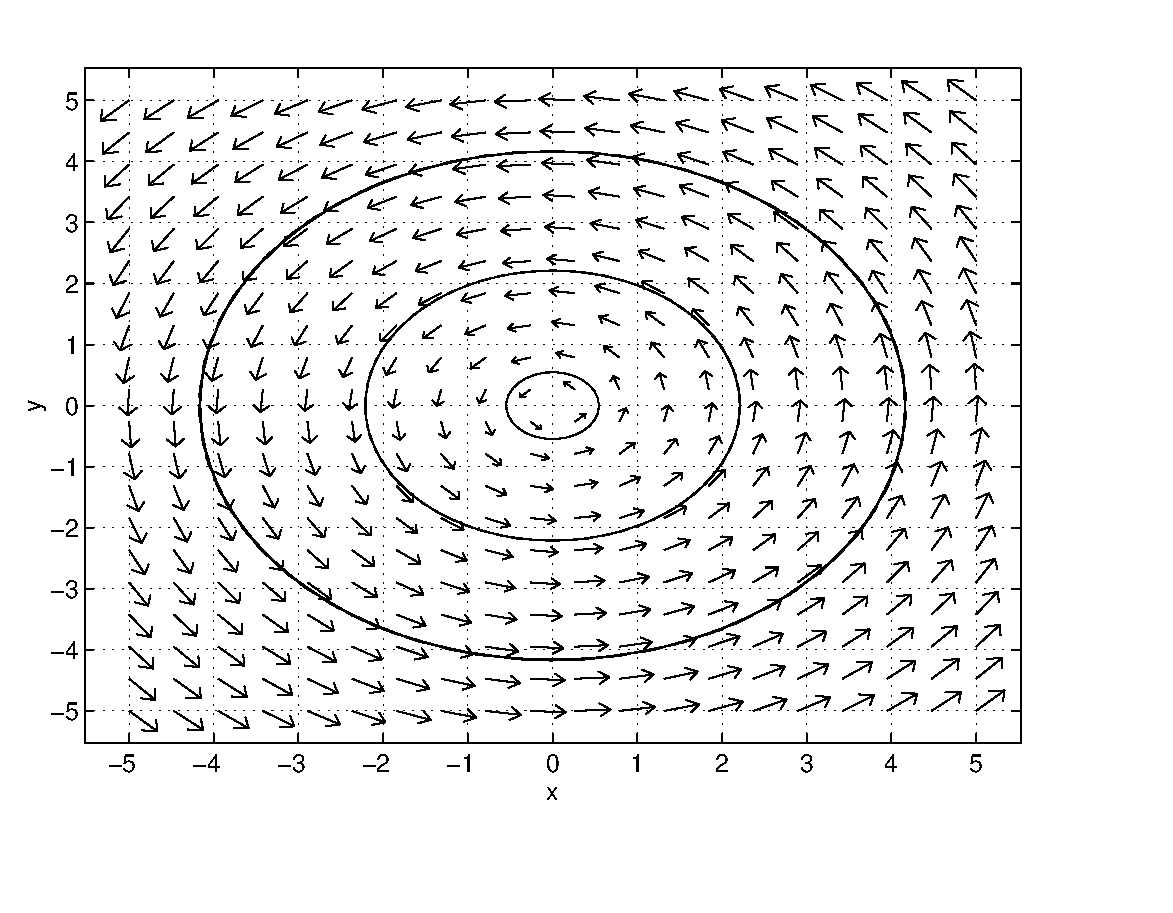
\psfig{file=../figures/center.eps,width=2.2in}
     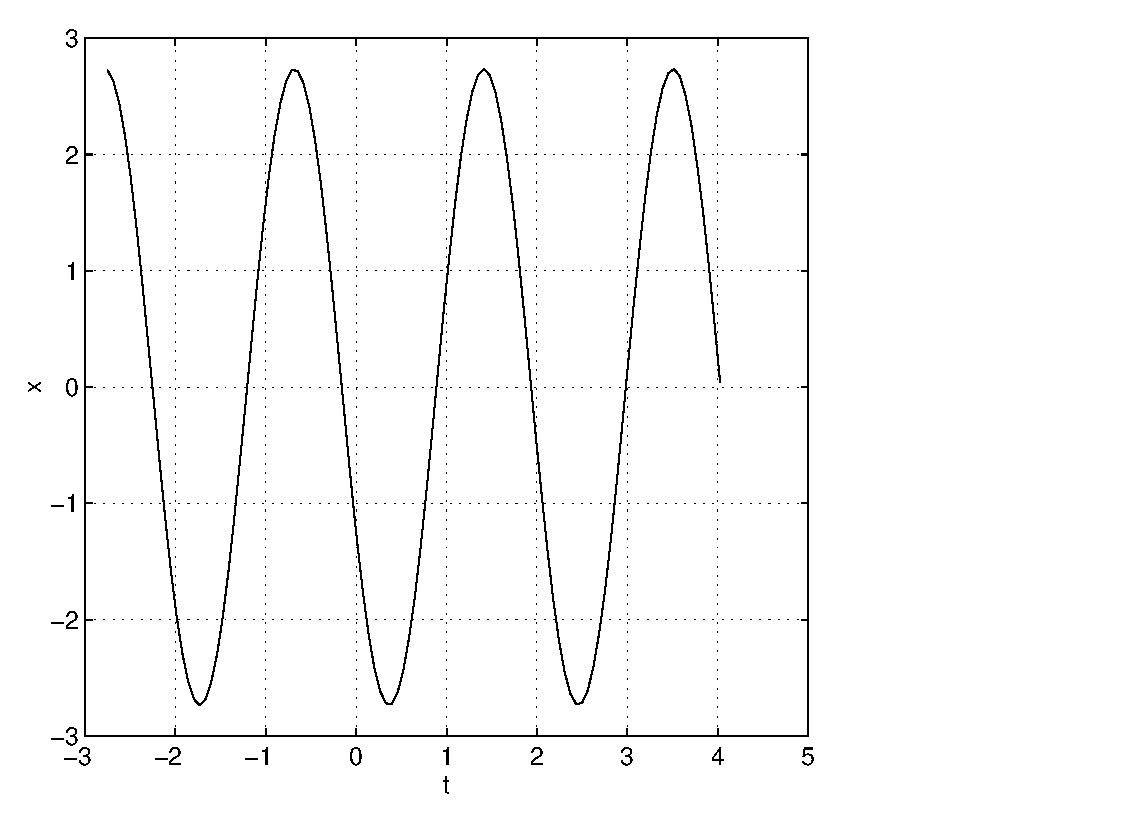
\psfig{file=../figures/centerts.eps,width=2.2in}}
     \caption{(Left) Solutions to $\dot{X}=BX$ for $\tau=3$.
	(Right) Time series of a solution illustrating time periodicity.}
     \label{F:center}
\end{figure*}

It is instructive to see how solutions change when the real part of the
eigenvalue traverses through zero.  Suppose that $C$ has eigenvalues
$\sigma\pm i\tau$ and is in normal form
\[
C = \mattwo{\sigma}{-\tau}{\tau}{\sigma}.
\]
We illustrate this change by graphing the time series (of both $x$ and $y$
versus $t$) in Figure~\ref{F:spiraling} with $\tau=3$ and $\sigma=-1,0,1$,
respectively. Note that when $\sigma<0$ the time series oscillate about zero
but also damp down to zero, while when $\sigma>0$ the time series oscillate
and diverge.  When $\sigma = 0$, there is an exact balance leading to time
periodic solutions.

\begin{figure*}[htb]
     \centerline{%
     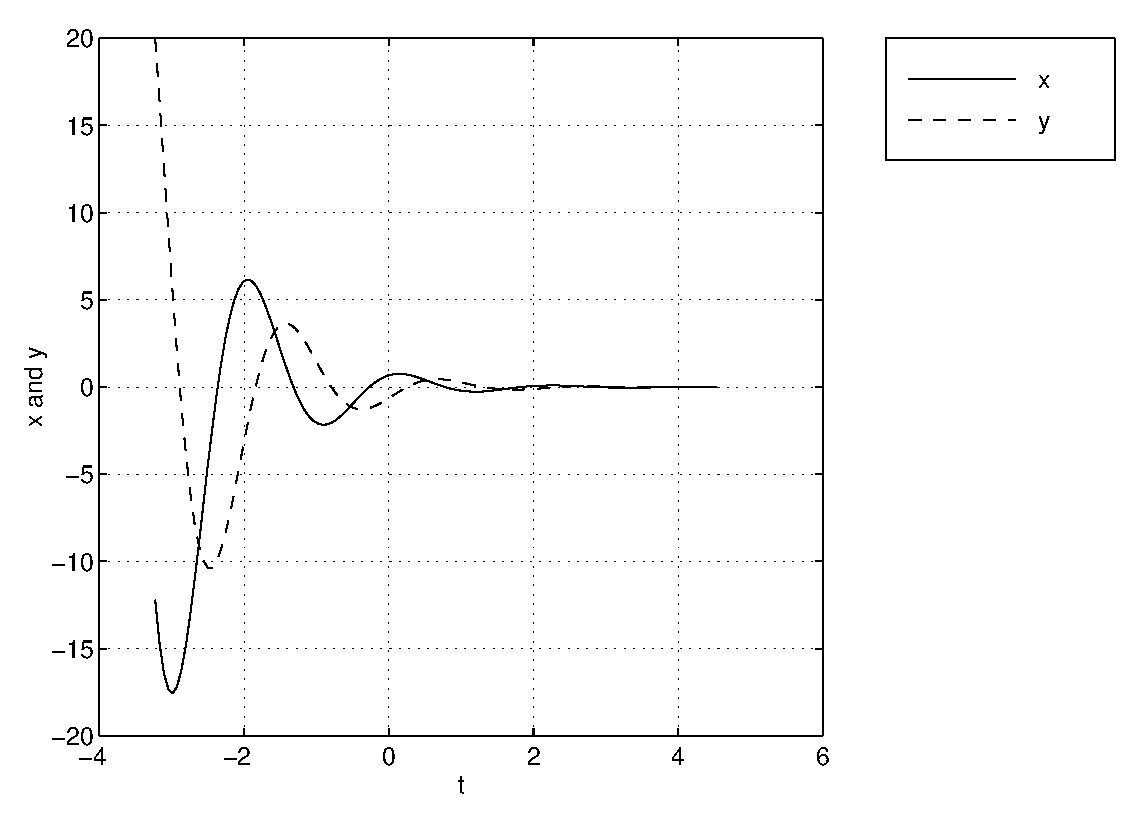
\psfig{file=../figures/spn1.eps,width=2.2in}
     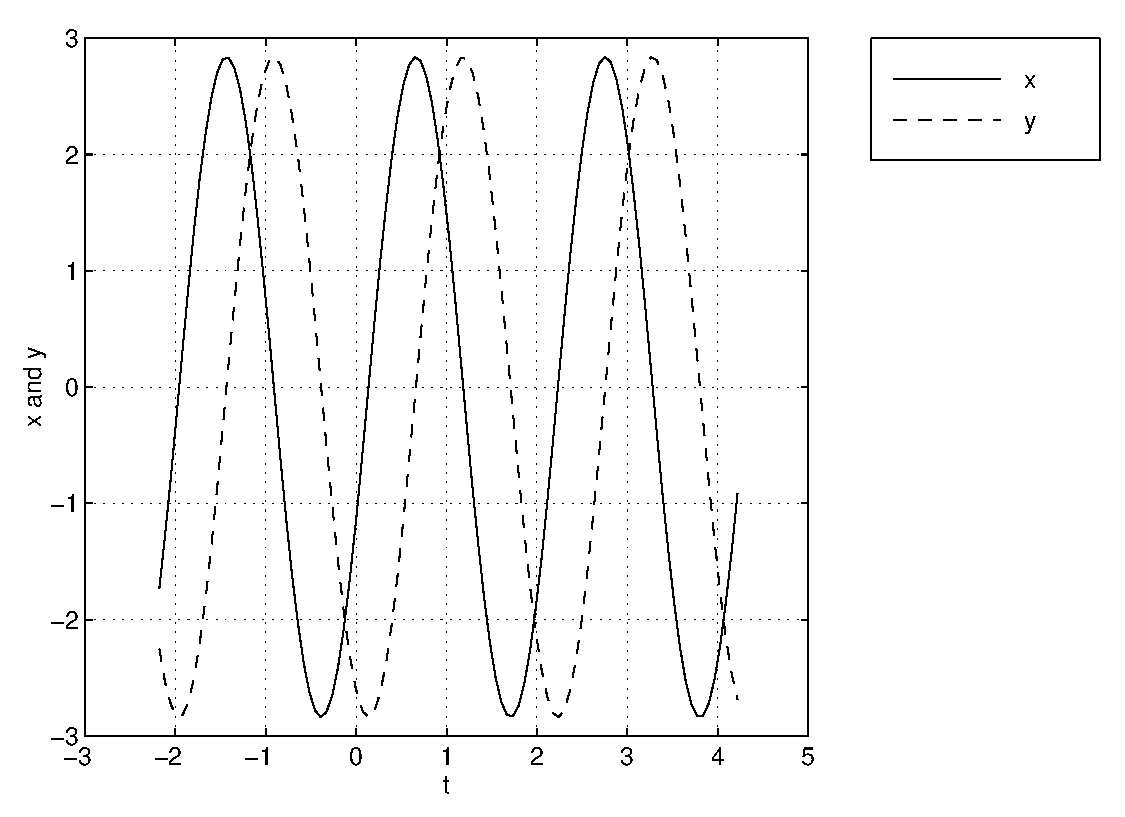
\psfig{file=../figures/sp0.eps,width=2.2in}
     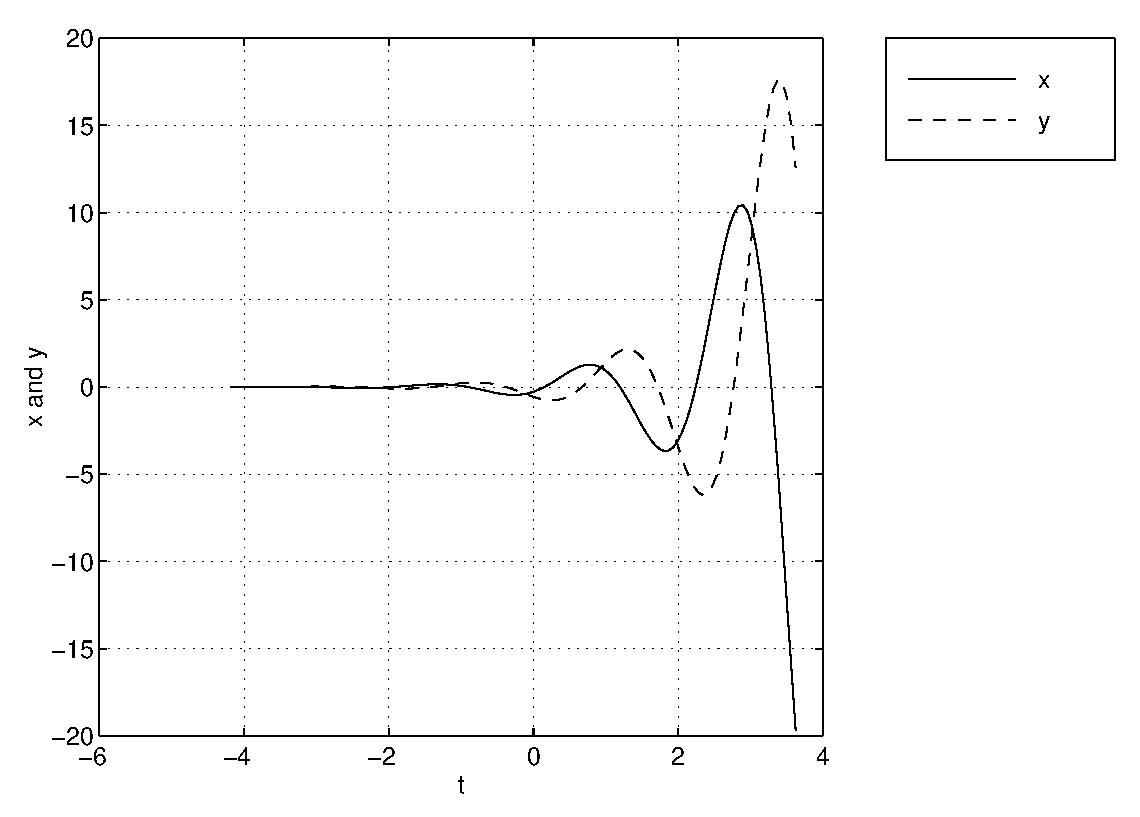
\psfig{file=../figures/sp1.eps,width=2.2in}}
     \caption{Solutions of $\dot{X}=BX$ for $\tau=3$ and $\sigma=-1,0,1$.}
     \label{F:spiraling}
\end{figure*}

\subsubsection*{Saddle Nodes}

When the determinant of a matrix $C$ is zero, then $C$ must have a zero
eigenvalue.  The simplest way for $\det(C)$ to be zero is for $C$ to have a
single zero eigenvalue.  In this case we call the origin a {\em saddle node}.

So the eigenvalues of a saddle node are $\lambda_1=0$ and $\lambda_2\neq 0$.
For simplicity of discussion, we assume that $\lambda_2<0$.  Let $v_1$ and
$v_2$ be the associated eigenvectors.  Since $Cv_1=0$, it follows that saddle
nodes have a line of equilibria\index{line of equilibria}
$X(t)=\alpha_1v_1$ for every scalar $\alpha_1$.

There is also a solution $X(t)=e^{\lambda_2 t}v_2$ that converges to the
origin in forward time (since $\lambda_2<0$).  The general solution to this
system is
\[
X(t) = \alpha_1 v_1 + \alpha_2 e^{\lambda_2 t}v_2,
\]
for scalars $\alpha_1$ and $\alpha_2$.  Since $\lambda_2<0$ this solution
converges on the equilibrium $\alpha_1 v_1$ in forward time.  Moreover,
the trajectory for any solution stays for all time on the line parallel
to the vector $v_2$.  The phase portrait\index{phase!portrait!for a saddle
node}
for the system
\begin{equation}  \label{e:10ev}
\frac{dX}{dt} = \mattwo{-2}{4}{1}{-2} X
\end{equation}
is shown in Figure~\ref{F:10ev} (left) along with the time series
of a solution (right).  Note how the time series (of $x$ versus $t$)
asymptotes onto the $x$ coordinate of an equilibrium.

\begin{figure*}[htb]
     \centerline{%
     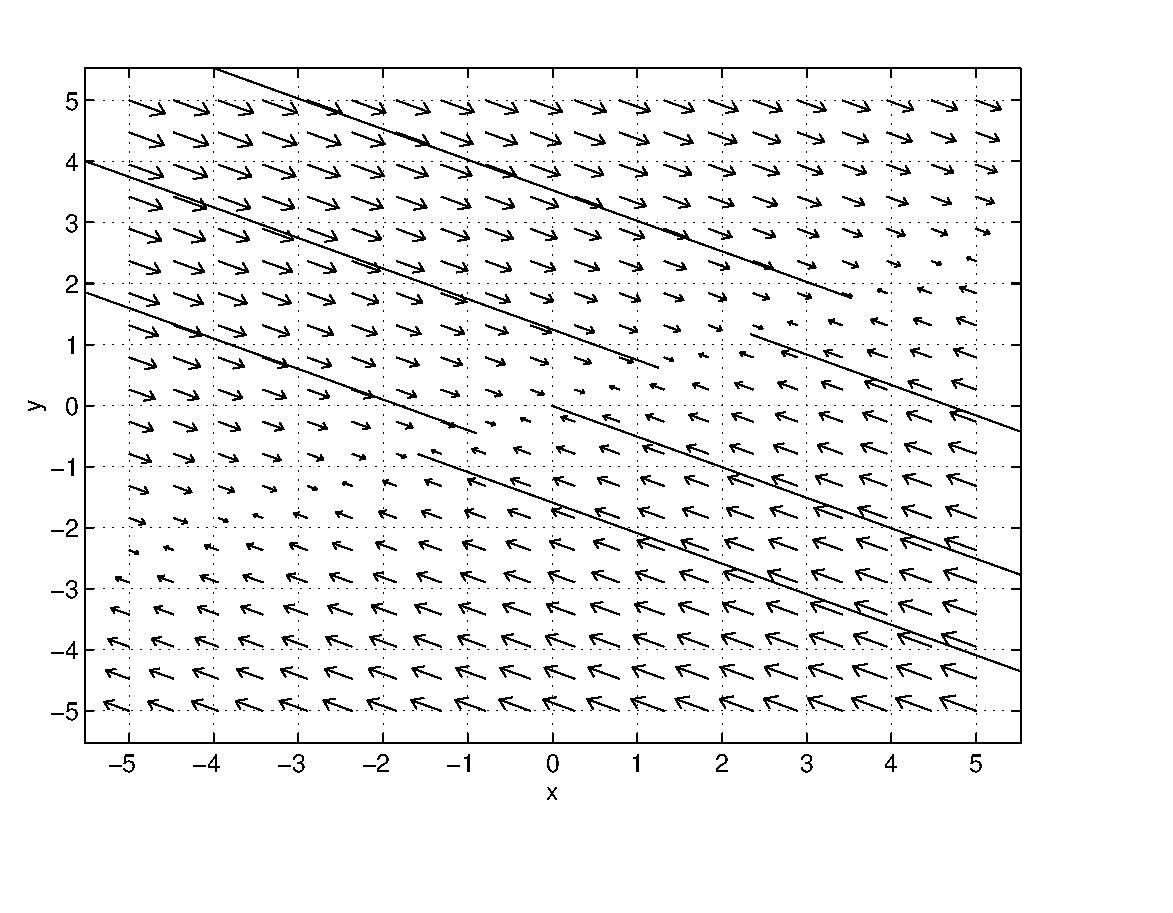
\psfig{file=../figures/z1ev.eps,width=2.2in}
     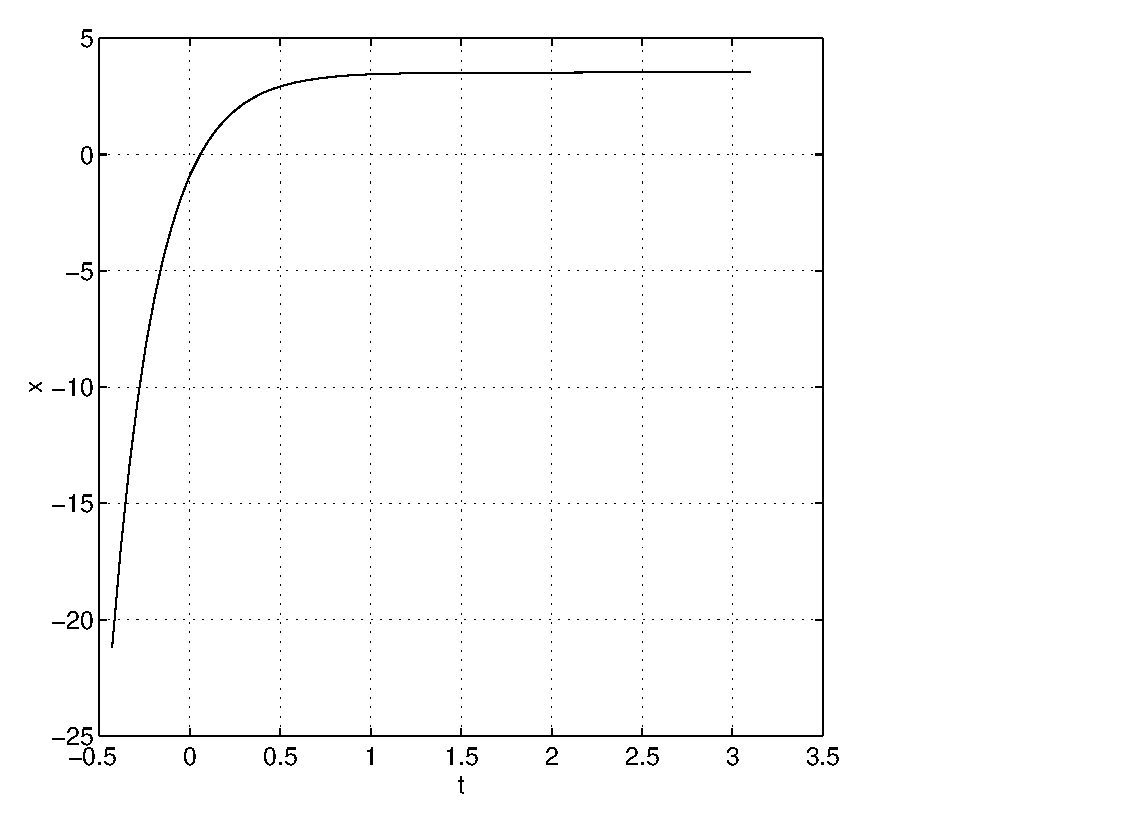
\psfig{file=../figures/z1evts.eps,width=2.2in}}
     \caption{(Left) Phase portrait of \protect\Ref{e:10ev}.
	(Right) Time series of a solution.}
     \label{F:10ev}
\end{figure*}

The saddle-node\index{saddle-node} is a
nonhyperbolic equilibrium\index{equilibrium!nonhyperbolic}
that sits between
the hyperbolic saddle and the hyperbolic node (either the nodal
sink or the nodal source), just as the center\index{center} sits
between the hyperbolic spiral source and the hyperbolic spiral sink.  To
illustrate this point we show three time series in
Figure~\ref{F:saddlenodebif} for the system
\begin{equation}  \label{e:saddlenodebif}
\frac{dX}{dt}  =  \mattwo{\mu}{0}{0}{-1}X
\end{equation}
when $\mu<0$, $\mu=0$, and $\mu>0$.  See how the $y$ time series
decays exponentially to zero in forward time in each case.  But
the $x$ time series converges to zero when $\mu<0$ and grows
exponentially when $\mu>0$.  Finally, when $\mu=0$ the $x$ time
series is constant.

\begin{figure*}[htb]
     \centerline{%
     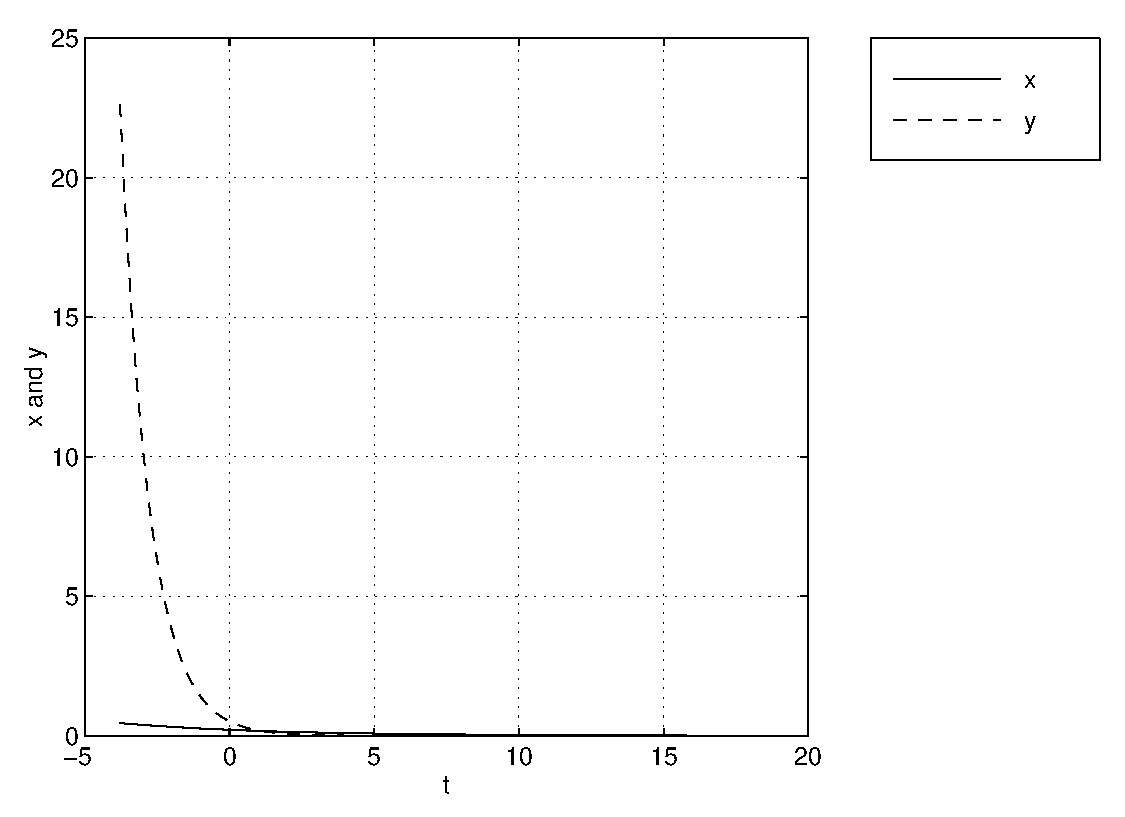
\psfig{file=../figures/snn1.eps,width=2.2in}
     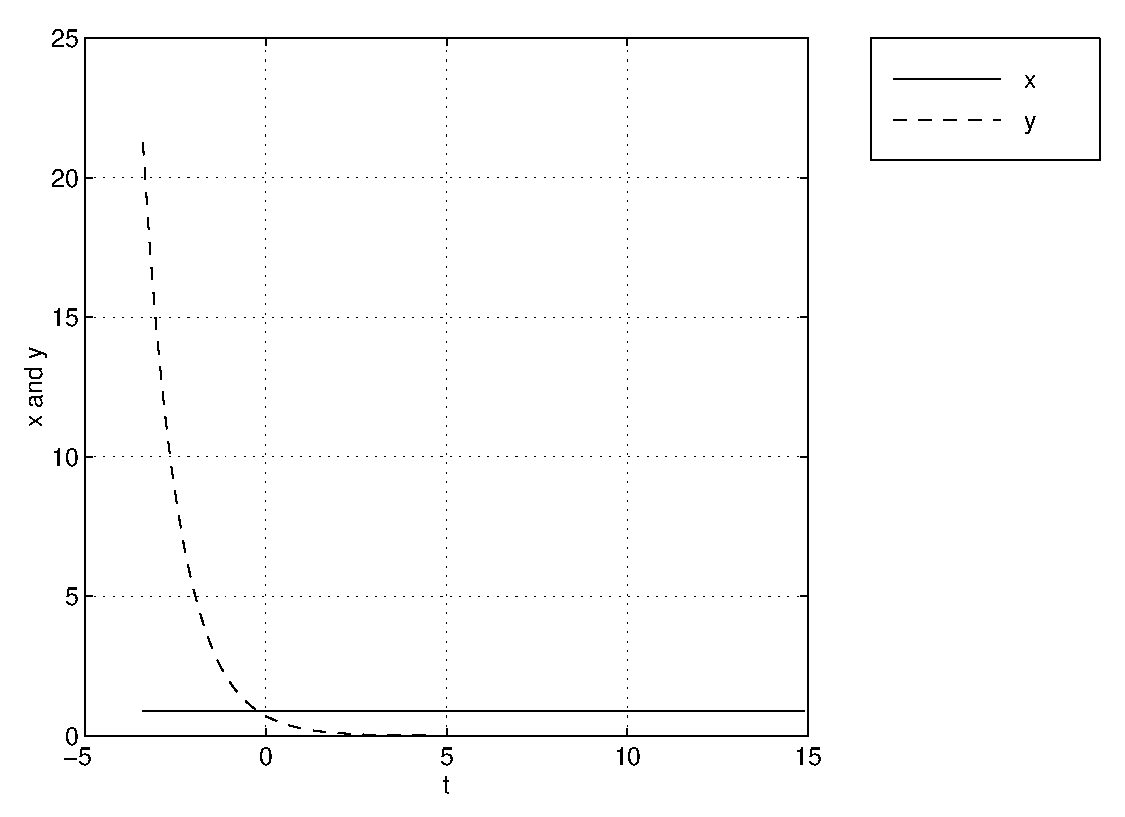
\psfig{file=../figures/sn0.eps,width=2.2in}
     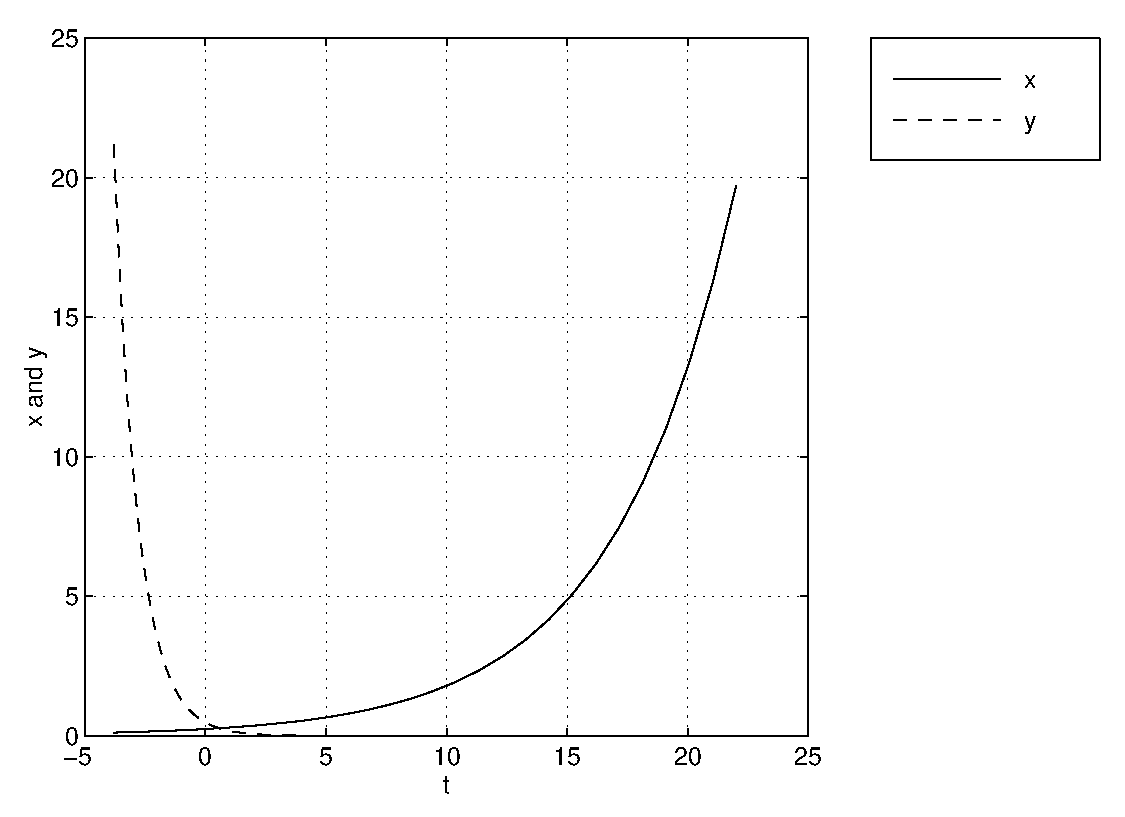
\psfig{file=../figures/snp1.eps,width=2.2in}}
     \caption{Time series for solutions of \protect\Ref{e:saddlenodebif}
	when $\mu=-0.2,0,0.2$.}
     \label{F:saddlenodebif}
\end{figure*}


\subsubsection*{Shears}
\index{shear}

The last example of a nonhyperbolic system occurs when the matrix $C$
has two zero eigenvalues --- but only one linearly independent
eigenvector.  In this case we call the origin a {\em shear\/}.  After a
similarity transformation such a system is
\begin{equation}  \label{e:00}
\frac{dX}{dt} = \mattwo{0}{1}{0}{0} X
\end{equation}
The solution is
\[
(x(t),y(t)) = (x_0+y_0t,y_0).
\]
Thus solutions move along lines parallel to the $x$ axis through
the point $(x_0,y_0)$ with speed $y_0$.  These trajectories move
to the right when $y_0>0$ and to the left when $y_0<0$.

\EXER

\TEXER

\noindent In Exercises~\ref{c6.9.1a} -- \ref{c6.9.1b}, find a $2\times 2$
matrix $C$ so that the differential equation $\dot{X}=CX$ satisfies the
given condition.
\begin{exercise} \label{c6.9.1a}
The origin is a center.
\end{exercise}
\begin{exercise} \label{c6.9.1b}
The origin is a saddle-node with equilibria on the line generated by the
vector $(-1,2)$.
\end{exercise}

\begin{exercise} \label{c6.9.2}
Recall from Chapter~\ref{Chap:Planar}, \Ref{ex:uspring} that the undamped
spring equation is $\frac{d^2x}{dt^2} + \kappa x = 0$, where $\kappa>0$.
\begin{itemize}
\item[(a)]   As a first order system this equation is:
\begin{eqnarray*}
\dot{x} & = & y \\
\dot{y} & = & -\kappa x.
\end{eqnarray*}
Sketch the phase portrait of this equation.
\item[(b)]  The damped spring equation, written as a first order system, is:
\begin{eqnarray*}
\dot{x} & = & y \\
\dot{y} & = & -\kappa x-\sigma y,
\end{eqnarray*}
where $\sigma>0$ is the damping.  Sketch the phase portrait of this equation.
\end{itemize}
\end{exercise}

\noindent In Exercises~\ref{E:PPa} -- \ref{E:PPe}, consider the four pictures
in Figure~\ref{F:PP}.  Each picture is a phase portrait of a system of
differential equations $\dot{X}=CX$ where $C$ is a $2\times 2$ matrix.  Answer
the given question for each of these phase portraits.
\begin{exercise}  \label{E:PPa}
What is the name of the type of equilibrium at the origin?
\end{exercise}
\begin{exercise}  \label{E:PPb}
Is the origin asymptotically stable?
\end{exercise}
\begin{exercise}  \label{E:PPc}
Is ${\rm trace}(C)$ positive, negative, or zero?
\end{exercise}
\begin{exercise}  \label{E:PPd}
Is $\det(C)$ positive, negative, or zero?
\end{exercise}
\begin{exercise}  \label{E:PPe}
Is ${\rm discriminant}(C)$ positive, negative, or zero?
\end{exercise}

\begin{figure*}[htb]
\centerline{(A) \hspace{2.7in} (B)}
           \centerline{%
           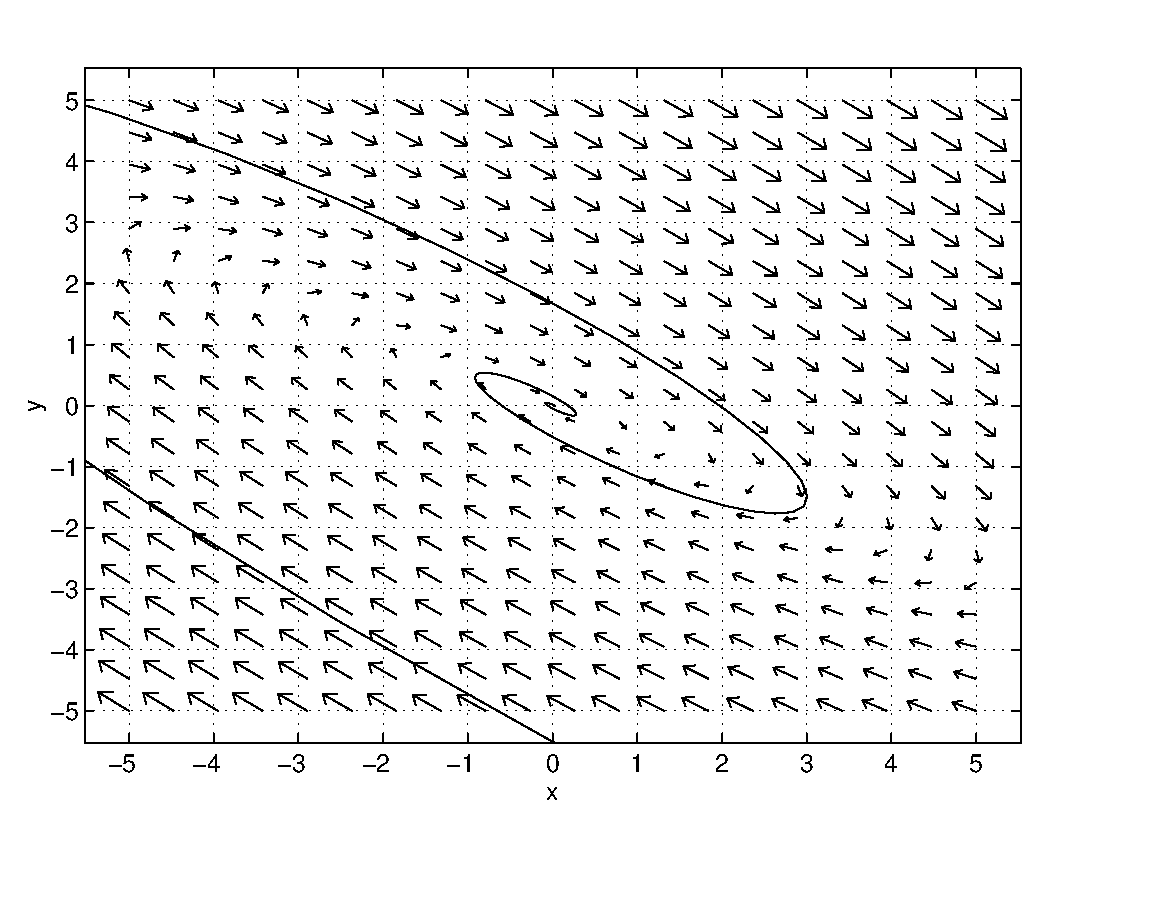
\psfig{file=../figures/e2B.eps,width=3.0in}
           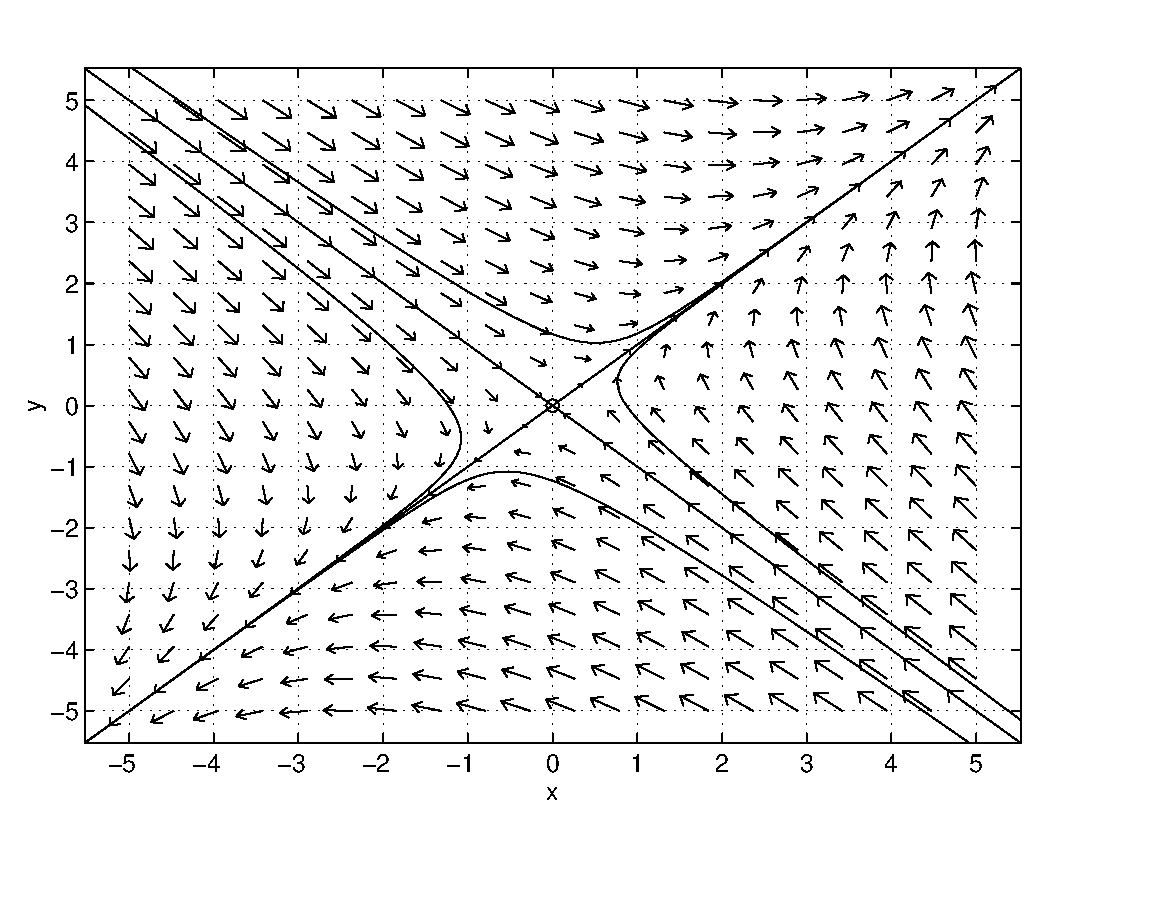
\psfig{file=../figures/e2C.eps,width=3.0in}}
\centerline{(C) \hspace{2.7in} (D)}
           \centerline{%
           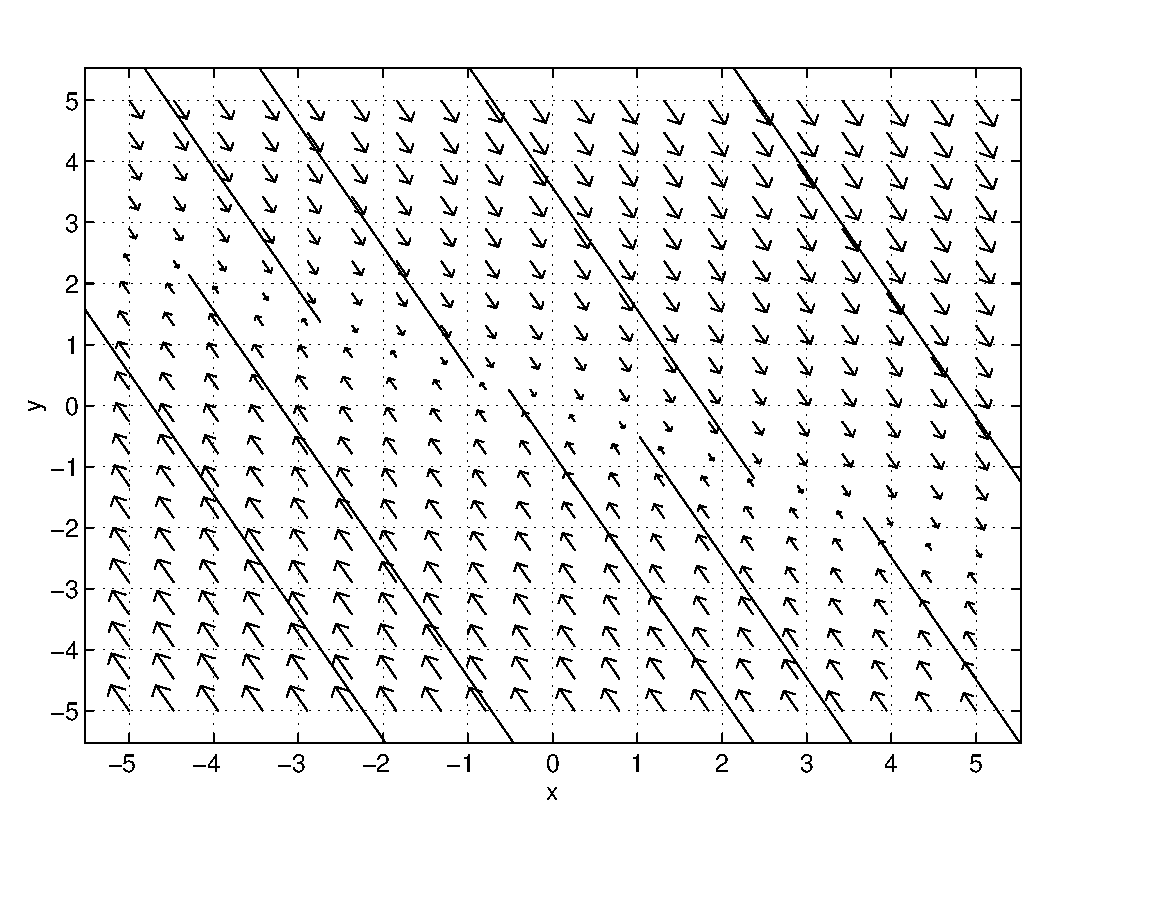
\psfig{file=../figures/e2A.eps,width=3.0in}
           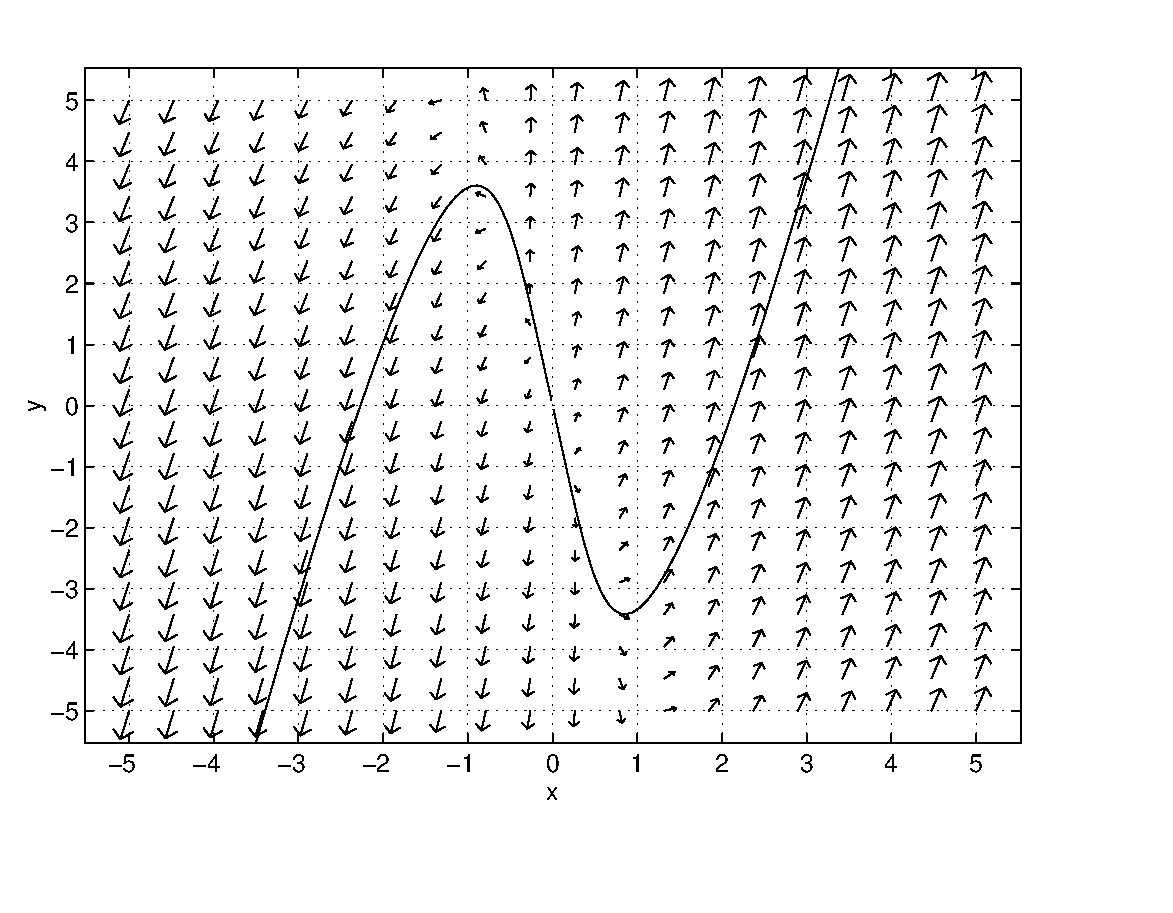
\psfig{file=../figures/e2D.eps,width=3.0in}}
\caption{Phase portraits for planar linear systems in
Exercises~\protect\ref{E:PPa} -- \protect\ref{E:PPe}}
\label{F:PP}
\end{figure*}

\noindent In Exercises~\ref{E:PQa} -- \ref{E:PQg}, consider the system of
differential equations $\dot{X}=CX$ where $C$ is the given matrix.  For each
system determine whether the origin is hyperbolic or not and the type of
equilibrium at the origin (spiral sink, center, etc.).
\begin{exercise}  \label{E:PQa}
$C = \mattwo{1}{-1}{2}{1}$.
\end{exercise}
\begin{exercise}  \label{E:PQb}
$C = \mattwo{1}{1}{-1}{1}$.
\end{exercise}
\begin{exercise}  \label{E:PQc}
$C = \mattwo{3}{-1}{1}{1}$.
\end{exercise}
\begin{exercise}  \label{E:PQd}
$C = \mattwo{1}{1}{1}{1}$.
\end{exercise}
\begin{exercise}  \label{E:PQe}
$C = \mattwo{2}{-2}{4}{-2}$.
\end{exercise}
\begin{exercise}  \label{E:PQf}
$C = \mattwo{2}{2}{-2}{-2}$.
\end{exercise}
\begin{exercise}  \label{E:PQg}
$C = \mattwo{1}{1}{4}{1}$.
\end{exercise}

\CEXER

\begin{exercise}  \label{E:notcircles}
Consider the system of differential equations $\dot{X}=CX$ where
$C=\mattwo{2}{-10}{1}{-2}$.  By hand show that this system is a center and
use {\sf pplane5} to determine its phase portrait.  Describe both the
similarities and the differences of the phase portrait of this system
and the phase portrait in Figure~\ref{F:center}.
\end{exercise}

\begin{exercise} \label{c6.9.5}
Consider the system of differential equations $\dot{X}=CX$ where
$C=\mattwo{2}{-4}{1}{-2}$.  By hand show that this system is a shear and
use {\sf pplane5} to determine its phase portrait.  Describe both the
similarities and the differences of the phase portrait of this system
and the phase portrait of \Ref{e:00}.
\end{exercise}

\end{document}
